\section{Señales con comportamiento en frecuencias variable}

\begin{frame}
\frametitle{Señales con comportamiento en frecuencia variable}
  \vspace{-0.2cm}
  \footnotesize

  \begin{itemize}
    \item Cuando se trabaja con señales reales, el comportamiento en frecuencia no tiene por que mantenerse a lo largo del tiempo.
    \item La DFT (o su implementaci\'{o}n como FFT) de una señal no permite caracterizar su cambio temporal de frecuencias, ya que determina el comportamiento en frecuencia de la señal completa.
    \item Para observar el cambio de de frecuencias a lo largo del tiempo, se puede:
    \begin{itemize}
      \footnotesize
      \item Trocear la señal y caracterizar, usando la FFT, el comportamiento en frecuencias de cada trozo.
      \item Utilizar alguna herramienta avanzada que permita realizar ese an\'{a}lisis de forma autom\'{a}tica: 
      \begin{itemize}
        \item El \alert{espectrograma}$^{1}$ es una buena elecci\'{o}n en muchos casos, ya que es una representaci\'{o}n gr\'{a}fica de la variabilidad temporal del comportamiento en frecuencia de una señal. 
        \item En concreto, utiliza un mapa de color para resaltar, en torno a que instantes de tiempo, las componentes en frecuencias m\'{a}s significativas (que tienen un m\'{o}dulo de FFT mayor)
      \end{itemize}
    \end{itemize}
  \end{itemize}
  \vspace{-0.2cm}
  \rule{12cm}{0.4pt}
  \scriptsize
  $^{1}$ El procedimiento que se sigue para obtener un espectrograma ser\'{a} explicado detenidamente  en el \'{u}ltimo tema de la asignatura 
\end{frame}


\begin{frame}
\frametitle{Espectrograma:  FFT a lo largo del tiempo}
\vspace{-0.2cm}
  \footnotesize

  \begin{itemize}
    \item Representaci\'{o}n de un espectrograma en Matlab: 
    \hspace{1cm} \color{blue}{\texttt{espectrogram(x,window,overlap,[],Fs)}}\color{black}
    \vspace{-0.1cm}

    \begin{itemize}
      \scriptsize
      \item \color{blue}\texttt{x}\color{black}: La señal muestreada
      \item \color{blue}\texttt{window}\color{black}: n\'{u}mero de elementos utilizados por cada FFT. 
      \item \color{blue}\texttt{overlap}\color{black}: n\'{u}mero de valores que se superponen. 
      \item \color{blue}\texttt{Fs}\color{black}: Frecuencia de muestreo. Se utiliza para representar correctamente las frecuencias en Hz y el paso temporal de la señal ($n \cdot T_s$).
      \vspace{0.3cm}
      \visible<2->{
      \begin{columns}[c]
        \begin{column}{5cm}
          \lstinputlisting{./Matlab/Spect4Corte.m}
        \end{column}
        \hspace{-0.8cm}\begin{column}{4cm}
          \scriptsize
          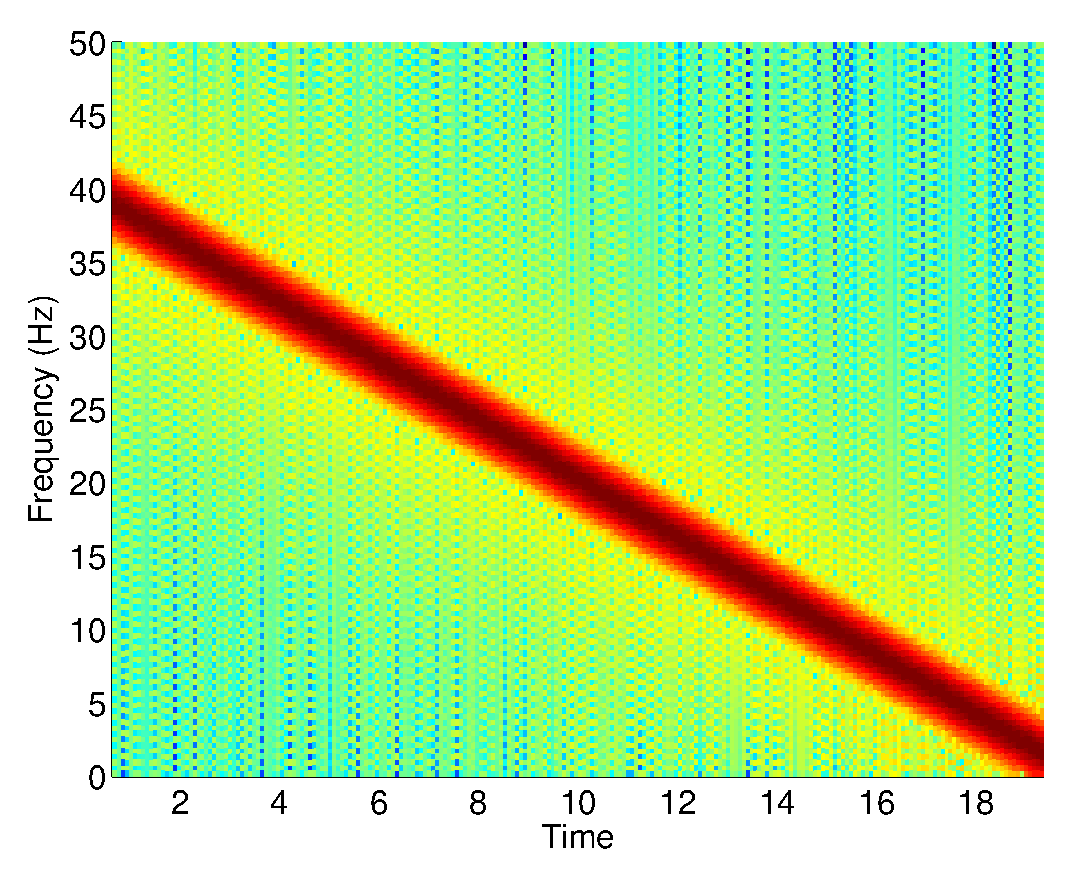
\includegraphics[width=4cm]{./Figures/Spect5.eps}
        \end{column}
      \end{columns}
      }
    \end{itemize}
  \end{itemize}
\end{frame}
